\documentclass[12pt]{article}

% Any percent sign marks a comment to the end of the line

% Every latex document starts with a documentclass declaration like this
% The option dvips allows for graphics, 12pt is the font size, and article
%   is the style




% array/table
\usepackage{array}
\usepackage{multirow}

% figure
\usepackage[pdftex]{graphicx}
\usepackage{epsfig}
\usepackage[hang]{subfigure}
\usepackage[small,bf]{caption}
\captionmargin=1.0cm


\usepackage{authblk}
\renewcommand\Authands{ and }

\usepackage[T1]{fontenc}
\usepackage[utf8]{inputenc}

%clickable ref
\usepackage[backref,pagebackref,naturalnames=true,colorlinks]{hyperref}



\setlength{\oddsidemargin}{0.25in}
\setlength{\textwidth}{6.5in}
\setlength{\topmargin}{0in}
\setlength{\textheight}{8.5in}



%----------------------------------------------------------------------------------------
%	DOCUMENT INFORMATION
%----------------------------------------------------------------------------------------

\title{EG01-23: CYCLUS Calculation Report}


\author[1]{B. MOUGINOT\thanks{\href{mailto:mouginot@wisc.edu}{mouginot@wisc.edu}}}
\author[1]{P.P.H. WILSON \thanks{\href{mailto:paul.wilson@wisc.edu}{paul.wilson@wisc.edu}}}
\author[1]{R. CARLSEN \thanks{\href{mailto:carlsen@wisc.edu}{carlsen@wisc.edu}}}
\affil[1]{University of Wisconsin-Madison, Department of Engineering Physics, CNERG group}


\date{\today}

\begin{document}
\maketitle

\section{Intro/specification}
The goal of this study is to model the transition from once-through PWRs (EG01) to full recycle FBRs (EG23). It appears that the immediate transition between the existing PWR fleet (EG01) and a full FBR fleet (EG23) was not directly possible. In order to have enough plutonium inventories to do the transition, a few LWRs must be deployed before starting to replace LWRs with FBRs. The deployment of the new LWRs and the FBRs was calculated to:
\begin{itemize}
\item minimize the amount of plutonium in the cycle,
\item follow the energy production requested (Fig 1b.).
\end{itemize}
The deployment schedule (Fig 1a.) has not been calculated using CYCLUS, it has been taken from B. Feng calculation and implemented in CYCLUS (with some approximation which will be detailed further in the document).

\begin{figure}[h!]
\centering
\subfigure[Deployment schedule]	{\epsfig{figure=img/CapacityStarted,width=0.48\textwidth}}
\subfigure[Electricity produced ]		{\epsfig{figure=img/ElectricityGenerated,width=0.48\textwidth}}
\caption{Deployment schedule and corresponding electricity produced by the different reactors where
R1(blue): existing PWR, R2(green): new builded PWR, R3(red): high FBR, R4(purple): low FBR.\label{fig:deployment} }
\end{figure}


\pagebreak
\section{Prototype configuration: what \& why}
This calculation is based on previous calculation operated by R. Carlsen, which can be found there. From this study, the configuration and deployment schedule of the separation facilities for PWR used fuel has been taken. The rest of the study has been adapted from it, to match B. Feng DYMOND calculation \cite{B.Feng_calculation}.

As Cyclus does not yet include direct support for on-demand processing, the separation and the fabrication have been modeled as follows to approximate on-demand separation, thus minimizing inventories of separated plutonium.
To achieve this, two differents calculations have been made. The first one correspond the modelization of a growing MOX fuel fabrication capacity following the MOX fuel requirement. The second one models both MOX fuel fabrication and fuel separation with limited capacities, which discreetly grow as the demand grows.

In both the reactor characteristic (core properties, fuel recipes, deployment schedule) are the same.
\subsection{Reactors}
After the PWR/FBR transition, new FBR reactor are deployed with a lower breeding ratio, in order to minimize the plutonium inventory. The properties of the differents reactor core used for the simulation have been summarized in Tab.\ref{tab:reactor}.\\


\begin{table}[h!]
\centering
\begin{tabular}{llll}
\hline
Core Properties		&	PWR 	&	FBR 1	&	FBR 2 	\\
\hline
Rated Power, [MWe]	&	1000		&	400		&	400		\\
Thermal Efficiency	&	N.A.		&	0.4		&	0.4		\\
Capacity Factor		&	0.90		&	0.90		&	0.90		\\
Number of batches	&	6		&	5		&	3		\\
Cycle length, [month]&	9		&	13		&	18		\\
Core Inventory, [tHM]&	14.784*6	&	7.524*5	&	11.466*3	\\
\hline
\end{tabular}
\caption{Reactor core properties.}
\label{tab:reactor}
\end{table}
Note that, because of the 1 month timestep of CYCLUS, some liberty has been taken with the coupled Batch-Quantity/Cycle-length in order to match as closely as possible with the specified quantities [REF-F.Bo]. The batches have been sized accordingly. All PWR reactors use enriched uranium fuel. The FBR used MOX fuel with different plutonium enrichments. The input/output fuel recipe are summarized in the Tab.\ref{tab:reactor_fuel} \cite{B.Feng_calculation}.

\begin{table}[h!]
\centering
\begin{tabular}{lllll}
\hline
\multicolumn{2}{c}{Reactor}			&	PWR [$\%w$]	&	FBR fuel 1  [$\%w$]	&	FBR fuel 2  [$\%w$] 	\\
\hline
\multirow{3}{*} {In recipe}	&	235U	&	95.8			&	0				&	0				\\
&	238U	&	4.2			&	92.36			&	91.466			\\
&	Pu		&	0			&	7.64				&	8.534			\\
\hline
\multirow{5}{*} {Out recipe}&	235U	&	0.8			&	0				&	0				\\
&	238U/U	&	92.68		&	85.99			&	86.025			\\
&	Pu		&	1.2			&	9.02				&	9.596			\\
&	MA		&	0.11			&	0.13				&	0.107			\\
&	FP		&	5.21			&	4.86				&	4.272			\\
\hline
\end{tabular}
\caption{Input/Output Fuel composition recipe for the different reactors. Note that for the FBR reactor fuel no isotopic distinctions have been made and U in FBR should be considered depleted uranium in the input recipes, the uranium isotopic change in the output recipes have not been investigated in this work.  }
\label{tab:reactor_fuel}
\end{table}

\subsection{Cooling/Storage}
After Irradiation, all fuel is sent to dedicated cooling storage, then they are transferred to a longer term storage after 84 month.
\subsection{Separation}

The LWR fuel separation is handled by three identical separation facilities, two deployed in 2030 and one in 2040. The FBR separation facilities have a very large separation capacity, in the first case, we have tried to limit the separation flux using the fuel fabrication facilities: since the fabrication if full as well as the separation, it will not request any more plutonium, so the separation will stop the separation...

\begin{table}[h!]
\centering
\begin{tabular}{lllll}
\hline
Separation Properties	&	PWR		&	FBR 1/2	\\
\hline
Throughput [tML]		&	83.3333	&	5000		\\
feed buffer [tML]		&	107.537	&	5000		\\
Pu output  [tML]		&	Unlimited	&	5000		\\
Pu separation efficiency	&	0.99		&	0.99		\\
Recycled Uranium [tML]	&	Unlimited	&	Unlimited	\\
U separation efficiency	&	0.99		&	0.99		\\
Waste [tML]			&	Unlimited	&	Unlimited	\\
\hline
\end{tabular}
\caption{Separation facilities core properties. }
\label{tab:separation_1}
\end{table}

\subsection{Fuel Fabrication}
The UOX fuel fabrication is handled by one enrichment facility, the properties of this enrichment facilities are summed up in Tab.\ref{tab:enrich_1}.

\begin{table}[h!]
\centering
\begin{tabular}{lllll}
\hline
Enrichment Properties	&	UOX		\\
\hline
Throughput [tML]		&	Unlimited	\\
swu capacity [tML]		&	1e97		\\
tails assay  			&	0.0025	\\
Initial feed [tML]		&	Unlimited	\\
\hline
\end{tabular}
\caption{Enrichment facilities properties. }
\label{tab:enrich_1}
\end{table}

The FBR fuel fabrication are suppose to handle and been deployed as a rate of 1 for 10 FBR reactors. Since the fuel composition and annual flux slightly change between FBR 1 and 2,, the specifications between fabrication are, as well, slightly differents... The detail of all fuel fabrication facilities characteristics can be found in Tab.\ref{tab:fuelfab_1}.

\begin{table}[h!]
\centering
\begin{tabular}{lllll}
\hline
Fuel Fab Properties	&	FBR 1	&	FBR 2	\\
\hline
Throughput [tML]	&	75.240	&	76.440	\\
depleted buffer [tML]	&	69.492	&	69.912	\\
Pu buffer  [tML]		&	5.748	&	5.856	\\
\hline
\end{tabular}
\caption{Fuel fabrication facilities properties.}
\label{tab:fuelfab_1}
\end{table}


\subsection{Results}
All fuel loading metrics (Fig.\ref{fig:RessourceUsed}) are the same or very close to the VISION simulations. Nevertheless one can observe some fluctuation on the annual fuel loading and the SWU requirement which are consistent with the batching of the initially deployed reactors which are synchronized.

\begin{figure}[h!]
\centering
\subfigure[Ressources Mined]			{\epsfig{figure=img/RessourceMined,width=0.48\textwidth}}
\subfigure[SWU Requirement]			{\epsfig{figure=img/SWURequierment,width=0.48\textwidth}}
\subfigure[Annual Fuel Loading Rate]	{\epsfig{figure=img/AnnualFuelLoading,width=0.48\textwidth}}
\caption{TBD.\label{fig:RessourceUsed} }
\end{figure}

The generated power and the deployment schedule (Fig. 3)  match perfectly the one of the VISION simulations. The sudden drop in 2210 is due to a lack of data after 2210: no new reactor have been started after this date.\\

\begin{figure}[h!]
\centering
\subfigure[Deployment schedule]	{\epsfig{figure=img/CapacityStarted,width=0.48\textwidth}}
\subfigure[Electricity produced ]		{\epsfig{figure=img/ElectricityGenerated,width=0.48\textwidth}}
\caption{Deployment schedule and corresponding electricity produced by the different reactors where
R1(blue): existing PWR, R2(green): new builded PWR, R3(red): high FBR, R4(purple): low FBR.\label{fig:deployment_bis} }
\end{figure}


The other curves are as expected. Indeed, the annual reprocessing rate correspond to the deployment :  for the UOX fuel start the reprocessing in 2010 with 2/3 of the capacity, and then an increase of 1/3 in 2030, and then a constant reprocessing rate (UOX1 + UOX2) until the end of the production of used UOX (all PWR decommissioning).


\begin{figure}[h!]
\centering
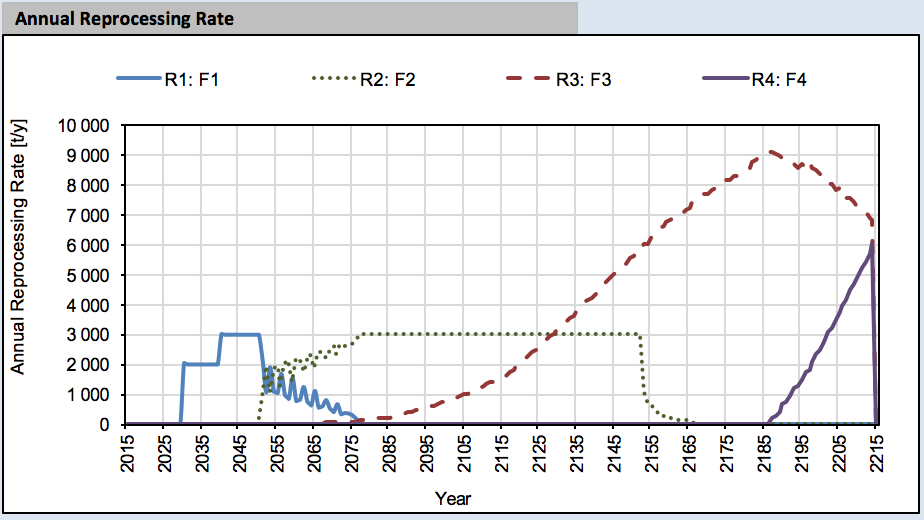
\includegraphics[width=0.62\textwidth]	{img/AnnualReprocessingRate_1}
\caption{Annual Reprocessing Rate.}
\label{fig:reprocessing_1}
\end{figure}


For the MOX fuel produced by the 2 different FBR types, it follows the loading of fresh fuel, with some shift : the reprocessing facility are greedy : they reprocess all the used fuel available. In consequence there is no FBR used fuel in storage they are directly reprocess after the cooling.


\begin{figure}[h!]
\centering
\subfigure[Used Fuel in Cooling]		{\epsfig{figure=img/usedFuelInCooling,width=0.48\textwidth}}
\subfigure[Fuel waiting for reprocessing]	{\epsfig{figure=img/UNFWaitingReprocessing_1,width=0.48\textwidth}}
\caption{TBD.\label{fig:cool_reprocc} }
\end{figure}


Concerning the fuel in storage, as almost all FBR used fuel are directly reprocess after cooling, all quantity barely stop increasing after all the UOX fuel have been reprocess.

\begin{figure}[h!]
\centering
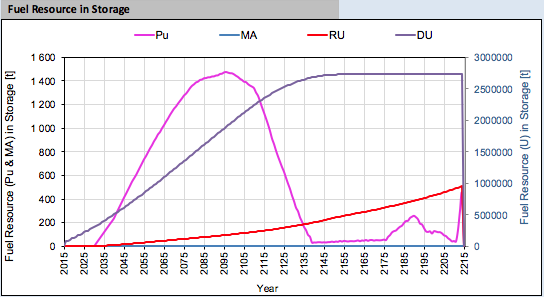
\includegraphics[width=0.62\textwidth]{img/FuelInStorage_1}
\caption{Storage Fuel composition.}
\label{fig:storagecompo_1}
\end{figure}

It appears that the capacity of the FBR fuel reprocessing are not enough to reprocess the full income of MOX fuel until 2195: this explain the some appearance of MOX fuel in storage waiting for reprocessing. With the deployment of the low breeder FBR, the high breeder reactor are decommissioned decreasing the incoming irradiated MOX fuel,  the reprocessing capacity is again higher than the sued MOX (type 1) production...


As shown in the figure \ref{fig:FC_Z} \& \ref{fig:WR_Z}, the quantity of plutonium in the storage follow the variation of the amount of MOX1 fuel in the storage.

\begin{figure}[h!]
\centering
\subfigure[Storage Fuel composition (zoomed)\label{fig:FC_Z}]		{\epsfig{figure=img/FuelInStorage_1_zoom,width=0.48\textwidth}}
\subfigure[Fuel waiting for reprocessing (zoomed)\label{fig:WR_Z}]	{\epsfig{figure=img/UNFWaitingReprocessing_1_zoom,width=0.48\textwidth}}
\caption{TBD.\label{fig:FC_WR_zoom} }
\end{figure}

\section{On demand Mimic Calculation}
In parallel of the previous calculation, I have tried to perform a calculation, where the separation facilities have limited capacities and are deployed accordingly to the plutonium requirement for MOX fuel fabrication. This deployment schedule is not perfect, but it provides a good idea to how should evolve such kind of calculation...
The only difference with the previous calculation is the way to define the reprocessing.

For this calculation, all fuel are reprocessed by only one kind of reprocessing facility. The fuel input preferences has been set to 3 to all irradiated UOX fuel, 2 for MOX fuel irradiated in high breeder, and 3 for the low breeder fuel (higher the number is higher the preferences is). The characteristic of those reprocessing facilities are summed up in Tab.\ref{tab:fuelfab_2}.

\begin{table}[h!]
\centering
\begin{tabular}{ll}
\hline
Separation Properties	&	All Fuel	\\
\hline
Throughput [tML]		&	60		\\
feed buffer [tML]		&	66		\\
Pu output  [tML]		&	6		\\
Pu separation efficiency	&	0.99		\\
Recycled Uranium [tML]	&	Unlimited	\\
U separation efficiency	&	0.99		\\
Waste [tML]			&	Unlimited	\\
\hline
\end{tabular}
\caption{Separation facilities core properties.}
\label{tab:fuelfab_2}
\end{table}


As in the calculation definition the only differences in the results can be observed in the behavior of the reprocessed fuel, the UNF fuel waiting for reprocessing and the composition of the storage, as the reprocessing process directly impact them.

\begin{figure}[h!]
\centering
\subfigure[Annual Reprocessing Rate]			{\epsfig{figure=img/AnnualReprocessingRate_2,width=0.48\textwidth}}
\subfigure[Fuel waiting for reprocessing]			{\epsfig{figure=img/UNFWaitingReprocessing_2,width=0.48\textwidth}}
\subfigure[Storage Fuel composition]	{\epsfig{figure=img/FuelInStorage_2,width=0.48\textwidth}}
\caption{TBD.\label{fig:ARR_FWR_SFC_2} }
\end{figure}

Indeed, as observed on Fig. 8a., the reprocessing follow the plutonium need of the FBR fuel fabrication. The UOX irradiated fuel only contain about only 1\% of plutonium, when FBR irradiated contain about 10\%, explaining the sudden decrease of the  amount of fuel reprocessed when switching from UOX fuel reprocessed to FBR fuel.
Because of both the reprocessing priority and "on demand" reprocess deployment, we can observed more fuel waiting for reprocessing, with a sudden consumption around 2125. We can also observe some of FBR fuel waiting for reprocessing, which decrease slowly, showing a well designed FBR deployment schedule...
\section{Summary}
This study have shown the capacity of CYCLUS to properly simulate a transition such as EG01 to EG23 transition.\\
The main observable differences are in the reprocessing and the storage of the used fuel, where it was not clear how it was managed in VISION. So even if I have been able to reproduce the overall calculation perform with B. Feng, some uncertainty remain on the exact signification of some data, like difference between UNF waiting for reprocessing and storage.\\
Despite CYCLUS is not able now to handle exact on demand behavior, it is possible to deploy the different facilities with limited capacities following the material demand to mimic a on demand behavior, as shown in the second calculation.

We can also observe some small difference in the pattern of fuel loading ( and almost all the reactor fuel metric), this comes from the way to model the batch in CYCLUS where in VISION all entities are managed with incoming and outgoing continuous flux.




%----------------------------------------------------------------------------------------
%	BIBLIOGRAPHY
%----------------------------------------------------------------------------------------

\bibliographystyle{unsrt}

\bibliography{}

%----------------------------------------------------------------------------------------


\end{document}